Consider a signal $x(t)$ sampled with a sampling interval $\Delta t$ to produce an infinite set of points $\{ x_n \}$.
We consider the \newword{discrete time Fourier transform} (DTFT) of this signal at frequency $\nu$, which is defined as
\begin{equation}
X(\nu) =\sum_{n=-\infty}^\infty x_n e^{-i 2\pi \nu n \Delta t} \, .
\end{equation}
Note that $\nu$ is a continuous frequency parameter.

To understand the properties of the DTFT, we compute its relation to the continuous time Fourier transform of $x(t)$.
First, we write $x_n$ in terms of the Fourier transform $\tilde{x}$
\begin{equation}
x_n \equiv x(n \Delta t) = \int \, df \, \tilde{x}(f) e^{i 2 \pi f n \Delta t} \, .
\end{equation}
Inserting this into the DTFT gives
\begin{equation}
X(\nu) = \sum_{n=-\infty}^\infty \int \, df \,
\tilde{x}(f) e^{i 2 \pi n \Delta t (f - \nu)} \, .
\end{equation}
Now we use a special property of sums of exponential functions,\footnote{This is directly related to the very useful Poisson summation formula.}
\begin{equation}
\sum_{n=-\infty}^\infty e^{i 2 \pi n q} =
\sum_{m=-\infty}^\infty \delta (m - q)
\end{equation}
to find
\begin{align}
X(\nu)
&= \sum_{m=-\infty}^\infty \int \, df \, \tilde{x}(f) \delta( m - \Delta t (f - \nu) ) \nonumber \\
  &= \sum_{m=-\infty}^\infty \tilde{x} \left( \nu + \frac{m}{\Delta t} \right) \, . \label{eq:aliasing}
\end{align}
Equation~(\ref{eq:aliasing}) tells us everything about the DTFT.
There are two critical points to understand.

First the DTFT separates frequency space into a set of bands; the $m^\text{th}$ band covers frequencies in the range
\begin{equation}
\left[ \frac{m}{\Delta t}, \, \frac{m+1}{\Delta t} \right] \, . \nonumber
\end{equation}
The DTFT values $X(\nu)$ are identical from band to band.
To see this, first note that any frequency $\nu$ can be uniquely expressed as $\nu = \mu + p / \Delta t$ where \mbox{$0 < \mu < 1/\Delta t$} is a frequency in the base band called the \newword{image frequency} and $p$ is an integer called the \newword{band index}.
Figure \ref{fig:aliasing}\,a illustrates this construction.
Using this representation for the DTFT frequency, we find
\begin{align}
  X \left(\mu + \frac{p}{\Delta t} \right) \nonumber
  &= \sum_{m=-\infty}^\infty \tilde{x}	\left(\mu + \frac{m + p}{\Delta t} \right) \nonumber \\
  &= \sum_{m=-\infty}^\infty \tilde{x}	\left(\mu + \frac{m}{\Delta t} \right) \nonumber \\
  &= X(\mu)
\end{align}
where the second line follows by shifting the sum index and the final line follows from Eq.~(\ref{eq:aliasing}).
Therefore, all of the information of the DTFT is contained within any one band, so we can limit discussion of the DTFT to one band.
By convention, we pick the \newword{base band} with $m=0$.
The bands and equality of $X(\nu)$ within each band are illustrated in Figure \ref{fig:bands}.

% \quickfig{\columnwidth}
% {bands.pdf}
% {The DTFT produces bands of with $1/\Delta t$.
% For \emph{any} $x_n$, the values of $X(\nu)$ within each band are identical.}
% {fig:bands}

\begin{figure*}[t]
  \begin{centering}
    
\includegraphics[width=\textwidth]{bands.pdf}
  \par\end{centering}
  \caption{The DTFT produces bands of with $1/\Delta t$. For \emph{any} $x_n$, the values of $X(\nu)$ within each band are identical.}
  \label{fig:bands}
\end{figure*}

Second, consider a signal $x(t) = \exp(i 2 \pi f t)$ which is sampled to $x_n = \exp( i 2 \pi f n \Delta t)$.
Expressing the signal frequency $f$ in terms of its image frequency and band index, $f= \mu + p/\Delta t$, we find
\begin{align}
X(\nu)
  &= \sum_{n=-\infty}^\infty x_n e^{-i 2 \pi \nu n} \nonumber \\
  &= \sum_{n=-\infty}^\infty e^{i 2 \pi (\mu - \nu) n \Delta t} \underbrace{e^{i 2 \pi p n}}_1 \nonumber \\
  &= \sum_{m=-\infty}^\infty \delta \left(\nu - \left[ \mu - \frac{m}{\Delta t} \right] \right) \nonumber \\
  &= \delta(\nu - \mu)
\end{align}
where in the last line we kept only the term $m=0$ because it is the only one in the base band and we showed above that the base band contains all of the information in the DTFT.
The value of $p$ does not show up in $X(\nu)$.
In other words, the DTFT of a complex sinusoid always shows up at its image frequency regardlyess of the band in which the underlying continuous signal sits, as illustrated in Figure \ref{fig:aliasing}\,a.
This effect is called \newword{aliasing}.
The words ``alias'' refers to an alternative identity; in this case, signals at frequencies outside the base band get an alternative identity at their image frequency within the base band.

Aliasing manifests in several ways.
Figure \ref{fig:aliasing}\,a shows the simplest case in which a single high frequency tone appears at its image frequency in the base band.
Now consider a signal with a continuous and infinitely extended frequency spectrum $\tilde{x}$, which we call the ``analog signal''.
Each frequency component produces an image in the base band.
In the simplest case wherein the support of $\tilde{x}$ sits exactly within a single DFTF band, the spectrum is exactly reproduced in the base band.
However, if the support of $\tilde{x}$ spans the boundary between two bands, then the DTFT splits the spectrum at the band boundary and places them in the opposite order in the base band, as illustrated in Figure \ref{fig:aliasing}\,b.
If the width of the support of $\tilde{x}$ is less than $1/\Delta t$, the images of the red and blue parts of the analog spectrum do not overlap in the base band, and it is possible to reconstruct the original signal from the DTFT, up to an overall frequency shift by $p/\Delta t$.
If the support of $\tilde{x}$ is greater than $1/\Delta t$ then the images of $\tilde{x}$ overlap in the base band, as shown in Figure \ref{fig:aliasing}\,c.
In this case, information about $\tilde{x}$ is lost and there is no way to reconstruct the original signal from the DTFT.

\quickfig{\columnwidth}{aliasing.pdf}{Aliasing. a) Under the action of the DTFT, a complex analog sinusoid shows up in all bands.
Since, we focus on $X(\nu)$ in the base band, we see the alias of the analog signal at frequency $\mu$.
b) If the analog signal's spectrum spans multiple DTFT bands, the DTFT (in the base band) appears to swap the high (blue) and low (red) frequency halves.
c) If the support of $\tilde{x}$ is wider than $1/\Delta t$ then the images from different parts of $\tilde{x}$ overlap in the DTFT bands.
The blue and red arrows indicate frequency components with the same image frequencies.}
{fig:aliasing}

Aliasing happens because analog sinusoids which differ in frequency by an integer multiple of $1/\Delta t$ yield exactly the same discrete samples, as shown in Figure \ref{fig:aliasing_sampling}.

\quickfig{\columnwidth}{aliasing_sampling.pdf}{Aliasing occurs when two different signals yield the same discrete samples.
a) Two complex sinusoids with frequencies $0.2/\Delta t$ (blue) and $1.2/\Delta t$ (red) are sampled with a sampling interval $\Delta t = 1$.
Solid lines indicate the real parts while broken lines indicate the imaginary parts.
Black circles show the samples of the real parts and black squares show the samples of the imaginary parts.
b) Same as construction, but with frequencies $0.4/\Delta t$ (blue) and $-0.6/\Delta t$ (red).
}
{fig:aliasing_sampling}

So far, our discussion of aliasing focused on complex sinusoids (as in Figure~\ref{fig:aliasing}\,a) and general continuous spectra (as in Figure~\ref{fig:aliasing}\,b and c).
We now consider the case of a real valued sinusoid as this case is the most often relevant in practical situations, and carries an extra subtlety.
Consider the real valued analog signal $x(t) = \cos(2 \pi f t)$ which is sampled to $x_n = \cos(2 \pi f n \Delta t)$.
To understand the DTFT of this signal we rewrite it in terms of its complex parts
\begin{equation}
x_n = \frac{1}{2} \left( e^{i 2 \pi f n \Delta t} + e^{-i 2 \pi f n \Delta t} \right) \, .
\end{equation}
The DTFT is linear, so the DTFT of this $x_n$ is the superposition of the DTFT's produced by each complex sinusoid component.
As shown above, each complex sinusoid produces a delta function in the base band.
If the analog signal frequency is $f = \mu + p/\Delta t$, then the image frequencies of the two complex sinusoids are $\mu$ and $1/\Delta t - \mu$, as illustrated in Figure \ref{fig:aliasing_real}.
These two images are related via reflection about the midpoint of the base band, called the \newword{Nyquist frequency}.
Therefore, real sinusoids at frequencies $\mu + p/\Delta t$ and $(p+1)/\Delta t - \mu$ yield the same DTFT and so only \emph{half} of the base band contains unique information.

% \quickwidefig{1.75\columnwidth}{aliasing_real.pdf}
% {Aliasing of a real valued sinusoid.
% Solid vertical arrows indicate the analog components while dotted vertical arrows represent their images.
% We show cases where the analog frequency sits in the base band, i.e. the band index of the analog signal is zero.
% a) The analog signal frequency $\mu$ sits in the lower half of the base band.
% Note that aliasing of the \emph{negative} frequency component $-\mu$ creates a base band image at $1/\Delta t - \mu$.
% This image looks like the component at $\mu$ mirrored about the midpoint of the base band.
% b) Here the analog signal frequency sits in the upper half of the base band.
% The alias of the negative frequency component sits at $\mu$, which again is the original base band signal mirrored about the mid point of the base band.
% Note that the DTFT's in these two cases are identical.
% }
% {fig:aliasing_real}

\begin{figure*}[h]
  \begin{centering}
    
\includegraphics[width=\widewidth\columnwidth]{aliasing_real.pdf}
  \par\end{centering}
  \caption{Aliasing of a real valued sinusoid.
Solid vertical arrows indicate the analog components while dotted vertical arrows represent their images.
We show cases where the analog frequency sits in the base band, i.e. the band index of the analog signal is zero.
a) The analog signal frequency $\mu$ sits in the lower half of the base band.
Note that aliasing of the \emph{negative} frequency component $-\mu$ creates a base band image at $1/\Delta t - \mu$.
This image looks like the component at $\mu$ mirrored about the midpoint of the base band.
b) Here the analog signal frequency sits in the upper half of the base band.
The alias of the negative frequency component sits at $\mu$, which again is the original base band signal mirrored about the mid point of the base band.
Note that the DTFT's in these two cases are identical.}
  \label{fig:aliasing_real}
\end{figure*}

A sampling system can only uniquely resolve frequency components over a band whose width is equal to or smaller than the Nyquist frequency, as illustrated by Figure \ref{fig:aliasing_real_spectra} which shows two illustrations of analog frequency spectra and their resulting DTFT's.
As shown in Figure \ref{fig:aliasing_real_spectra}\,a, if the positive part of the analog spectrum occupies less than half a DTFT band (i.e. the analog bandwidth is less than the Nyquist frequency), then the DTFT image of the negative part of the analog spectrum does not overlap the positive part.
In this case, the DTFT in the lower half of the base band faithfully represents the original analog spectrum, and it is possible to reconstruct the continuous analog time signal from the discrete samples.

If the analog spectrum occupies a frequency region larger than half of a DTFT band (i.e. has a bandwidth larger than the Nyquist frequency), then the analog spectral components at frequencies related by reflection about the Nyquist frequency are summed in the DTFT, as illustrated in Figure \ref{fig:aliasing_real_spectra}\,b.
In this case there is no way to recover the original analog spectrum from the DTFT.

\begin{figure*}[h]
  \begin{centering}
    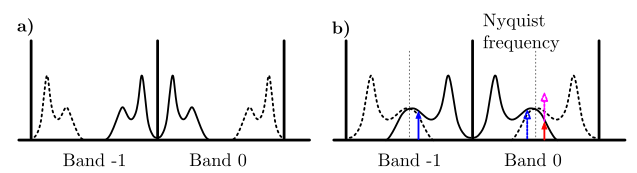
\includegraphics[width=\widewidth\columnwidth]{aliasing_real_spectra.pdf}
  \par\end{centering}
  \caption{Aliasing of real valued signals.
Solid curves indicate the original analog spectra, while the dotted curves indicate the images produced by the DTFT.
a) The positive part of the analog spectrum occupies less than half of a DTFT band.
The positive part of the analog spectrum and the base band image of the negative part of the analog spectrum do not overlap, so the lower half of the base band DTFT faithfully represents the original analog spectrum.
b) The positive part of the analog spectrum occupies more than half a band, so it overlaps with the base band image of the negative part.
The solid red arrow indicates a component in the positive part of the analog spectrum.
The solid blue arrow indicates a component in the negative part of the analog spectrum whose image frequency matches the red component.
The dotted purple arrow indicates the DTFT value at the red arrow's frequency, which is the sum of the solid red and solid blue components.
The dotted blue arrow indicates the part of the positive analog spectrum whose corresponding negative part's image has the same frequency as the red component.
Note that the solid red and dotted blue frequencies are related by reflection about the Nyquist frequency.}
  \label{fig:aliasing_real_spectra}
\end{figure*}

